\chapter{تنفيذ التكليف وتعبئة النماذج}
\label{ch:06-assignments}
\section{ابدأ من «التكليفات»}
\label{sec:assignments-start}

يجد الباحث كل عمله في «المهام» ثم «التكليفات» ثم «المطلوب مني». تُرتَّب البطاقات بحسب الموعد: «هذا الأسبوع»، ثم «لاحقاً»، ثم «بلا موعد». ولكل منشأة بطاقة واحدة تجمع وحدات الحزمة.

\begin{figure}[H]
\centering
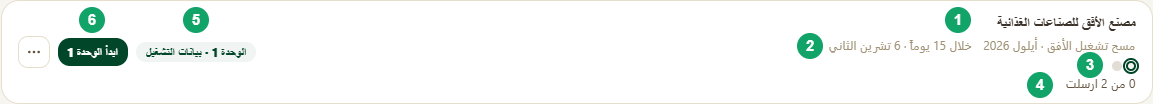
\includegraphics[width=\linewidth]{assets/screens/assignments-card-ar.png}
\caption{بطاقة مصنع الأفق في «المطلوب مني»}
\label{fig:assignments-card}
\shotnote{هذه البطاقة هي نقطة دخول عمر إلى المسح. تفيده في معرفة المنشأة والموعد والوحدة التالية دون أن يفتح شيئاً. ① اسم المنشأة. ② الحزمة والجولة، ثم الموعد. ③ نقطة لكل وحدة: الأولى مفتوحة، والثانية مقفلة. ④ «0 من 2 أُرسلت». ⑤ الوحدة التالية. ⑥ «ابدأ الوحدة 1».}
\end{figure}

في أعلى الصفحة يعرض «عمل اليوم» التكليفات التي يمكن تعبئتها دون اتصال، وزر «نزّل للعمل دون اتصال». نزّلها قبل الخروج إلى منطقة ضعيفة التغطية.

\begin{rcnote}[تطبيق المثال]
يفتح عمر «التكليفات» فيجد مصنع الأفق تحت «لاحقاً»: «مسح تشغيل الأفق · أيلول 2026»، و«خلال 15 يوماً · 6 تشرين الثاني»، و«0 من 2 أُرسلت». يضغط «ابدأ الوحدة 1».
\end{rcnote}

\section{املأ الصفحة الأولى}
\label{sec:assignments-first-page}

تُفتح الوحدة كإجابة جديدة برقم مسودة، مثل «\#-D-3». وفوق النموذج شريط الحزمة: اسم المنشأة، ورقم الوحدة، وما يُفتح بعد إرسالها.

\begin{figure}[H]
\centering
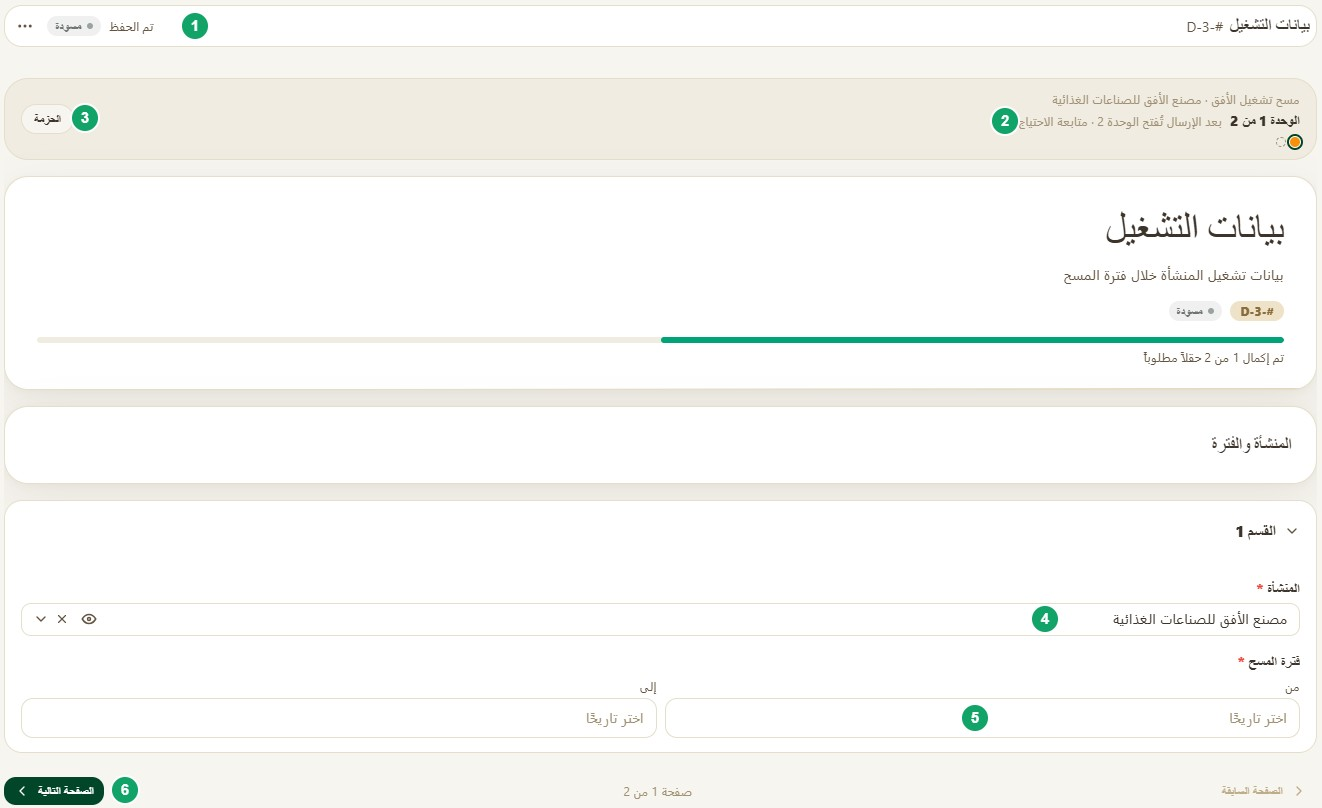
\includegraphics[width=\linewidth]{assets/screens/assignments-open-ar.jpg}
\caption{الوحدة الأولى عند فتحها}
\label{fig:assignments-open}
\shotnote{هذه أول شاشة يراها عمر بعد أن يبدأ الوحدة. تفيده في التأكد من أنه يعمل على المنشأة الصحيحة قبل أن يكتب أي رقم. ① «تم الحفظ» و«مسودة»: يحفظ النظام كل تغيير تلقائياً. ② شريط الحزمة: «الوحدة 1 من 2»، وبعد الإرسال تُفتح «متابعة الاحتياج». ③ «الحزمة»: صفحة كل وحدات المنشأة. ④ «المنشأة»: مملوءة من التكليف. ⑤ «فترة المسح». ⑥ «الصفحة التالية».}
\end{figure}

\begin{enumerate}
\item تأكد من اسم المنشأة. لا تغيّره؛ فهو يأتي من التكليف.
\item املأ الأسئلة المطلوبة، وعليها علامة *. ويعرض شريط التقدم عدد ما أكملته منها.
\item اضغط «الصفحة التالية».
\end{enumerate}

\begin{rcnote}[تطبيق المثال]
يجد عمر «مصنع الأفق للصناعات الغذائية» مملوءاً. يختار في «فترة المسح» من 1 إلى 30 أيلول 2026، فيظهر تحتها «30 يوماً»، ويصبح التقدم «تم إكمال 2 من 2 حقلاً مطلوباً».
\end{rcnote}

\section{املأ «التشغيل» وصحّح رسائل التحقق}
\label{sec:assignments-validation}

يتحقق النموذج من كل إجابة لحظة كتابتها. وإذا كانت القيمة خارج حدودها، يتلون الحقل بالأحمر وتظهر بجانبه رسالة تذكر الحد المسموح. صحح القيمة قبل الإرسال. وقد يظهر سؤال جديد بحسب إجابتك، كما ضبطنا في القسم~\ref{sec:forms-rules}.

\begin{figure}[H]
\centering
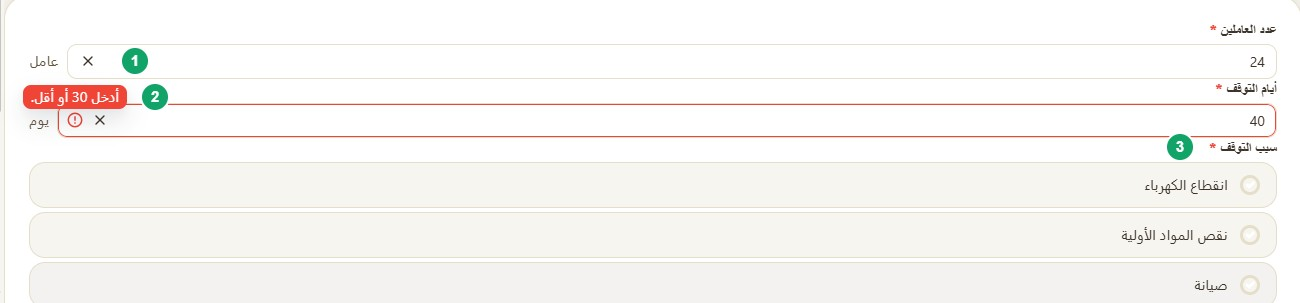
\includegraphics[width=\linewidth]{assets/screens/assignments-validation-ar.jpg}
\caption{رسالة تحقق في «أيام التوقف»}
\label{fig:assignments-validation}
\shotnote{تعرض الصورة القواعد التي بنيناها في الفصل الرابع وهي تعمل أثناء التعبئة. تفيدك في فهم سبب ظهور سؤال أو رفض قيمة. ① «عدد العاملين» ووحدته «عامل». ② الرسالة «أدخل 30 أو أقل.» لأن القيمة 40. ③ «سبب التوقف»: ظهر وصار مطلوباً، لأن أيام التوقف أكبر من 0.}
\end{figure}

\begin{table}[H]
\centering
\caption{ما يحدث مع كل قيمة لأيام التوقف}
\label{tab:assignments-stop-days}
\begin{tabularx}{\linewidth}{R{2.4cm} Y}
\rcHeaderRow
\thh{القيمة} & \thh{ما يظهر}\\
0 & لا يظهر «سبب التوقف»، والمطلوب سؤالان.\\
3 & يظهر «سبب التوقف» ويصبح مطلوباً، فيصير المطلوب ثلاثة أسئلة.\\
40 & يتلون الحقل بالأحمر وتظهر «أدخل 30 أو أقل.».\\
\end{tabularx}
\end{table}

\begin{rcnote}[تطبيق المثال]
يكتب عمر 24 في «عدد العاملين». ثم يكتب 40 في «أيام التوقف» خطأً، فتظهر الرسالة. يصححها إلى 3، فيختار في «سبب التوقف» «أخرى». يصبح التقدم «تم إكمال 3 من 3».
\end{rcnote}

\section{احفظ وعد لاحقاً}
\label{sec:assignments-draft}

لا يوجد زر «حفظ». فكل تغيير يُحفظ تلقائياً، وتظهر «تم الحفظ» أعلى النموذج. ويمكنك ترك الإجابة والعودة إليها في أي وقت قبل الإرسال.

\begin{enumerate}
\item ارجع إلى «التكليفات». يتغير زر البطاقة إلى «متابعة الوحدة 1».
\item اضغطه. تُفتح المسودة نفسها، وفيها كل ما كتبته.
\end{enumerate}

والمسودة لا تدخل مسار المراجعة؛ فالمراجعة تبدأ بالإرسال، كما في القسم~\ref{sec:observatory-approval-path}.

\begin{rcnote}[تطبيق المثال]
يغلق عمر النموذج بعد أن يكتب أيام التوقف، لينتقل إلى عمل آخر. يعود بعد ساعة إلى «التكليفات»، فيجد «متابعة الوحدة 1». يفتحها فيجد 24 و3 و«أخرى» كما تركها.
\end{rcnote}

\section{أرسل الوحدة}
\label{sec:assignments-submit}

\begin{enumerate}
\item في آخر صفحة، اقرأ التنبيه فوق زر الإرسال: ما الوحدة التي ستُفتح بعدها، وبأي شرط.
\item اضغط «إرسال الوحدة».
\item تسألك النافذة: «إرسال الطلب؟ لن تتمكّن من تعديله أثناء معالجته.» اضغط «إرسال الطلب».
\end{enumerate}

\begin{figure}[H]
\centering
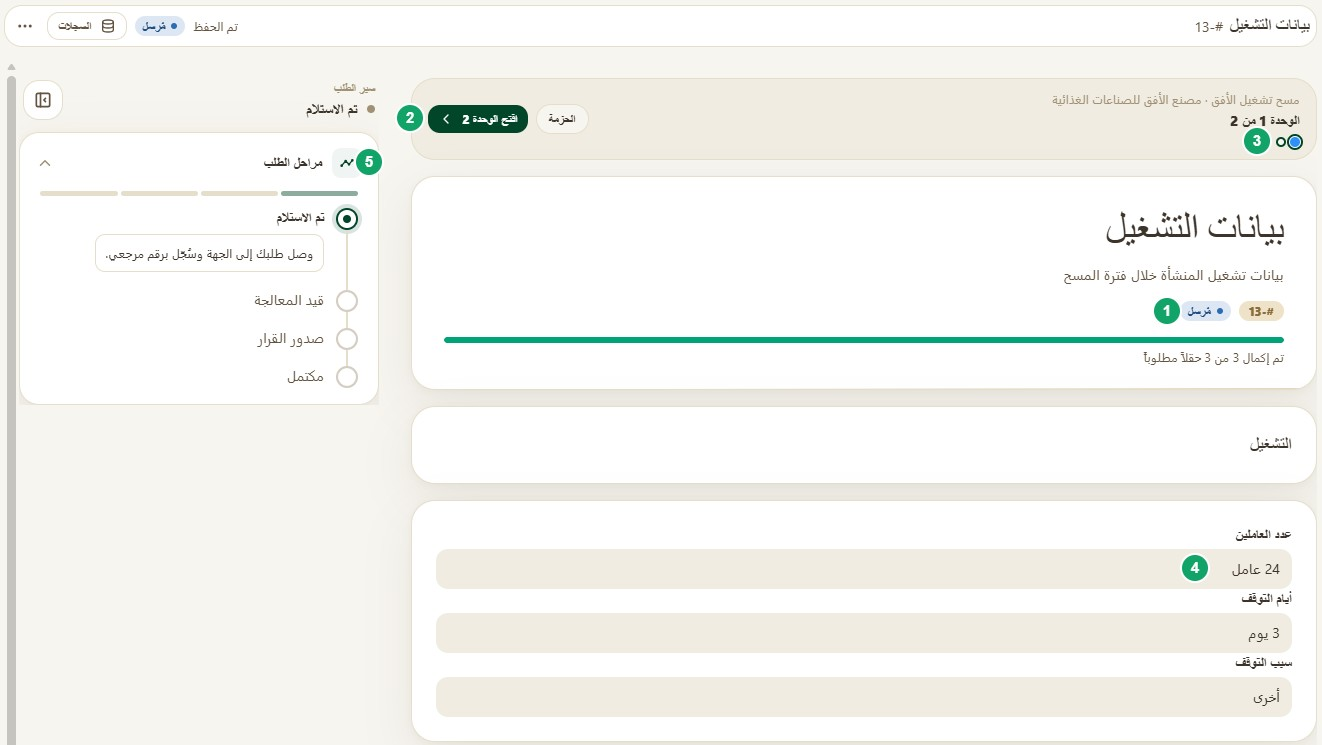
\includegraphics[width=\linewidth]{assets/screens/assignments-submitted-ar.jpg}
\caption{الوحدة الأولى بعد إرسالها}
\label{fig:assignments-submitted}
\shotnote{هذه حالة الإجابة بعد الإرسال مباشرة. تفيدك في التأكد من أن الإرسال تم، ومعرفة ما عليك بعده. ① الرقم النهائي «\#-13» بدل رقم المسودة، والحالة «مُرسل». ② «افتح الوحدة 2»: ظهر لأن شرطها تحقق. ③ نقطتا الوحدتين: الأولى مُرسلة، والثانية مفتوحة. ④ الإجابات للعرض فقط. ⑤ «مراحل الطلب»: الإجابة في «تم الاستلام».}
\end{figure}

بعد الإرسال لا تستطيع تعديل الإجابة. إذا اكتشفت خطأً، انتظر أن يعيدها المراجع للتصحيح، كما سنرى في الفصل~\ref{ch:07-review}.

\begin{rcnote}[تطبيق المثال]
يرسل عمر «بيانات التشغيل». يتغير الرقم من «\#-D-3» إلى «\#-13»، والحالة إلى «مُرسل». ولأن أيام التوقف 3، يظهر «افتح الوحدة 2». ولو كانت 0، لتخطّت الحزمة «متابعة الاحتياج».
\end{rcnote}

\section{أكمل الحزمة وتابعها}
\label{sec:assignments-package}

صفحة الحزمة تجمع وحدات المنشأة في مكان واحد. افتحها من زر «الحزمة» في أي وحدة، أو من «فتح الحزمة» في البطاقة.

\begin{figure}[H]
\centering
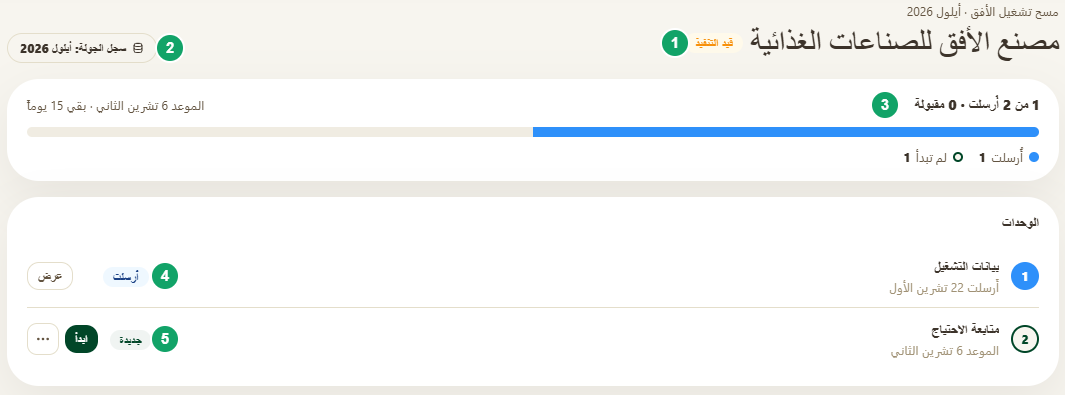
\includegraphics[width=\linewidth]{assets/screens/assignments-package-ar.png}
\caption{صفحة حزمة مصنع الأفق بعد إرسال الوحدة الأولى}
\label{fig:assignments-package}
\shotnote{تعرض الصفحة تقدم المنشأة في الجولة كلها. تفيدك في معرفة ما أُرسل وما بقي، دون التنقل بين الوحدات. ① الحالة «قيد التنفيذ». ② «سجل الجولة: أيلول 2026»، وقد أُنشئ عند التكليف. ③ «1 من 2 أُرسلت · 0 مقبولة»، والموعد. ④ الوحدة الأولى «أُرسلت»، ويمكن عرضها. ⑤ الوحدة الثانية «جديدة»، وزر «ابدأ».}
\end{figure}

\begin{rcnote}[تطبيق المثال]
يضغط عمر «ابدأ» أمام «متابعة الاحتياج». يختار «كهرباء ومولدات»، ويكتب: «مولّد احتياطي يغطي ساعات انقطاع الكهرباء»، ثم يرسل. تعرض الحزمة «2 من 2 أُرسلت · 0 مقبولة»، وتبقى «قيد التنفيذ». فالخطة تعدّ التكليف منتهياً عندما تصبح الإجابات «مقبولة»، أي بعد المراجعة.
\end{rcnote}

\begin{table}[H]
\centering
\caption{مشكلات التعبئة وحلولها}
\label{tab:assignments-problems}
\begin{tabularx}{\linewidth}{Y Y}
\rcHeaderRow
\thh{ما الذي لاحظته؟} & \thh{ماذا تفعل؟}\\
لا أجد المنشأة في «المطلوب مني» & اختر «مفتوحة»، وابحث في «لاحقاً» و«بلا موعد». وإن لم تجدها، راجع القسم~\ref{sec:observatory-role-check}.\\
حقل أحمر ورسالة بجانبه & صحح القيمة لتقع ضمن الحد المكتوب في الرسالة.\\
لا تُفتح الوحدة التالية & أرسل الوحدة الحالية أولاً. وقد تُتخطى الوحدة إذا لم يتحقق شرطها.\\
لا يظهر زر «إرسال الوحدة» & أبلغ مسؤول الحزمة؛ فالنموذج يحتاج إلى «تفعيل المسار» قبل نشره.\\
أريد تعديل إجابة بعد إرسالها & لا يمكن. انتظر إعادتها من المراجع، ثم صحح المعلَّم فقط.\\
\end{tabularx}
\end{table}

\begin{rcchecklist}[بعد أن ينهي عمر عمله]
\begin{checklist}
\item فتح المصنع من «التكليفات»، وتأكد من اسمه في الوحدة.
\item صحح رسالة «أدخل 30 أو أقل.»، وأدخل 24 عاملاً و3 أيام توقف.
\item عاد إلى المسودة من «متابعة الوحدة 1» ووجد قيمه محفوظة.
\item أرسل الوحدتين، وصار رقم الأولى نهائياً.
\item الحزمة تعرض «2 من 2 أُرسلت · 0 مقبولة».
\end{checklist}
\end{rcchecklist}

وصلت إجابتا عمر الآن إلى ليلى. في الفصل~\ref{ch:07-review} تراجعهما، وتعيد سبب التوقف «أخرى» للتصحيح.
